\section{Timer and Interrupts}

\subsection{Modulo Counter}

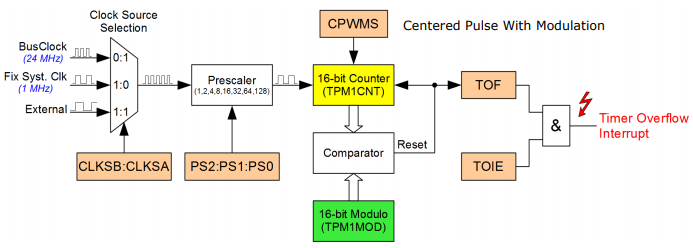
\includegraphics[width=0.5\textwidth]{timer-overview.png}

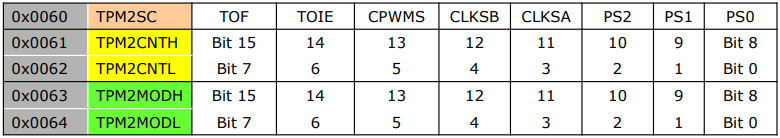
\includegraphics[width=0.5\textwidth]{timer-2-control-registers.png}

\subsection{Modulo Frequency}

$\mathbf{T_{TOF} = (MOD + 1) \cdot PS / f_{Clk}}$
\newline
\begin{itemize}
    \item{$\mathbf{T_{TOF}}$: Time between two Timer-Overflow events}
    \item{$\mathbf{MOD}$: Value of the Modulo set}
    \item{$\mathbf{PS}$: Presacler value}
    \item{$\mathbf{f_{Clk}}$: frequency of the controller}
\end{itemize}

\textit{
    \newline
    To calculate the modulo, the frequency (Clock Source) needs to be selected
    and the prescaler needs to be defined. To calculate the Modulo value, following can
    be used. The Modulo is 2 Bytes, so it needs to be between \textbf{0 < MOD < 65536}
    \newline
}

$\mathbf{MOD = (\frac{T_{TOF} \cdot f_{Clk}}{PS}) - 1}$

\subsection{Timer Control Registers}

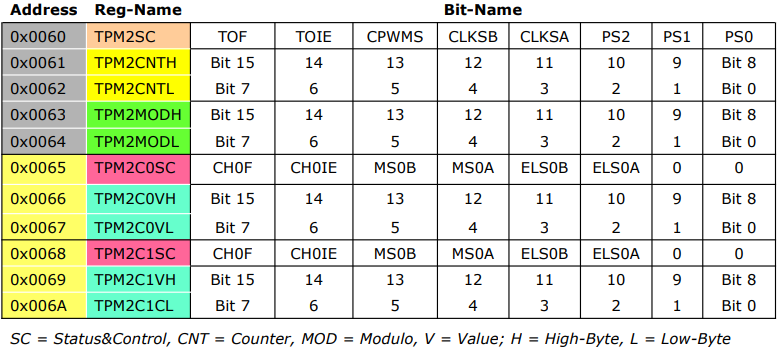
\includegraphics[width=0.5\textwidth]{timer-2-control-registers-channels.png}

\begin{lstlisting}
interrupt void myTofISR(void)
{
    // myTofISR function needs to be mapped
    // in the vectortable -> parameterfile (.prm).
    //reset the interrupt flag
    TPM1SC_TOF = 0;

    //run logic
}
void initTimer(void)
{
    //set module to 25780 / 0x64B4
    TPM1MODH = 0x64;
    TPM1MODL = 0xB4;
    //TPM1MOD = 25780;
    //Clock set to 1 MHz
    TPM1SC_CLKSA = 0;
    TPM1SC_CLKSB = 1;

    //define Prescaler to 128
    TPM1SC_PS0 = 1;
    TPM1SC_PS1 = 1;
    TPM1SC_PS2 = 1;

    // enable timer Overflow Interrupt
    // this should be the last action
    TPM1SC_TOIE = 1;
    // Reset the Timer Overflow Interrupt
    TPM1SC_TOF = 0;
}
void main(void)
{
    initTimer();
    //enable interrupts
    EnableInterrupts;
}
\end{lstlisting}

\subsection{Polling and Interrupts}

\textit{
    A MC-System has to react instantly to events (internal or external)
    (e.g. measure value monitoring, serial communication).\newline
    The \textbf{instant of time} of these events is \textbf{not known in advance}. \newline
    There are two ways to react to those kind of events: \newline
}

\begin{itemize}
    \item{
        \textbf{Interrupt} = Exception handling \newline
        \textit{
            enables \textbf{realtime capable} systems (depends on interrupt
            \textbf{latency}). \textbf{Fast reaction time} through automatic reaction
            to events and interrupt of the program to execute an
            Interrupt-Service-Routine (ISR). \newline
            Needs substancial effort for \textbf{state backup}, because the instant of
            the program interruption is unknown.
        }
    }
    \item {
        \textbf{Polling} = cyclic requesting \newline
        \textit{
            \textbf{Shorter} program \textbf{interruption}. Since the instant of time is
            known during programming, the state can be backed up more efficiently. \newline
            \textbf{Waste of caclulation time} if events occure rarely
        }
    }
\end{itemize}

\textit{
    \newline
    Each MCU holds an Interrupt-Logic to realise real-time systems.
}

\subsection{Save Interrupt State}

